\documentclass{beamer}
\usepackage{graphicx}
\usepackage[style=authoryear-icomp]{biblatex}
\usepackage{xcolor}
\usepackage{subcaption}
\usepackage{cancel}
\usepackage{graphviz}

% BEAMER SETUP
\usetheme{CambridgeUS}
\usecolortheme{rose}
\setbeamertemplate{footline}[frame number]
\usefonttheme[onlymath]{serif}

% DEFINE COMMANDS
\newcommand{\question}[1]{\textit{\textcolor{blue}{#1}}}
\newcommand{\todo}[1]{\textit{\textcolor{red}{#1}}}
\newcommand{\citationneeded}{\textbf{\color{blue}[Citation Needed]}}
\renewcommand{\footnotesize}{\fontsize{7pt}{2pt}\selectfont}
\DeclareMathOperator*{\argmin}{arg\,min} % thin space, limits underneath in displays

% PRESENTATION METADATA
\title[]{The Motion Primitives of Motions in Microseconds}
\author[]{Pravi Samaratunga}
\institute{Boston University ECE}
\date{\today}

\addbibresource{./assets/sources.bib}

\begin{document}
\begin{frame}
   \begin{center}
       \titlepage
     
       
\includegraphics[width=0.4\textwidth]{./assets/BU_logo.png}
   \end{center}
\end{frame}

\begin{frame}{Presentation Overview}
\begin{itemize}
\item Sampling-Based Motion Planning \\
\item Motion Primitives \\
\item \textit{Motions in Microseconds} \\
\item Strengths \& Weaknesses\\
\item Future Work \\
\end{itemize}
\end{frame}

\section{Introduction}
\subsection{\textsc{sbmp}}

\begin{frame}{Sampling-Based Motion Planning}

\pause
\begin{block}{What is Sampling-Based Motion Planning (\textsc{sbmp})?}
\pause Sampling-based motion planning \textsc{sbmp} is a method of determining how a robot moves through configuration space by sampling values from that space. %list off examples of algorithms, note tree-based vs graph-based
\end{block}

\pause
\begin{block}{Why is it relevant?} 
\pause \textsc{sbmp} algorithms are widely applicable and used in many fields. %list them off here
However, it can take several seconds for \textsc{sbmp} methods to execute, so there is ample space for innovation.
\end{block}

\pause
\begin{block}{How do we optimize \textsc{sbmp}?}
Over the years, many optimizations have been introduced to \textsc{sbmp}. We will discuss \textsc{vamp}, the Vector-Accelerated Motion Planning system as introduced by \cite{paper:MiM}.
\end{block}
\end{frame}

\begin{frame}{Example \textsc{sbmp} Execution: Problem Definition}
%\only<1>{Problem Definition}\only<2>{Step 1: Sample State Space}\only<3>{Step 2: Connect State to Graph}\only<4>{Step 3: Graph Search}
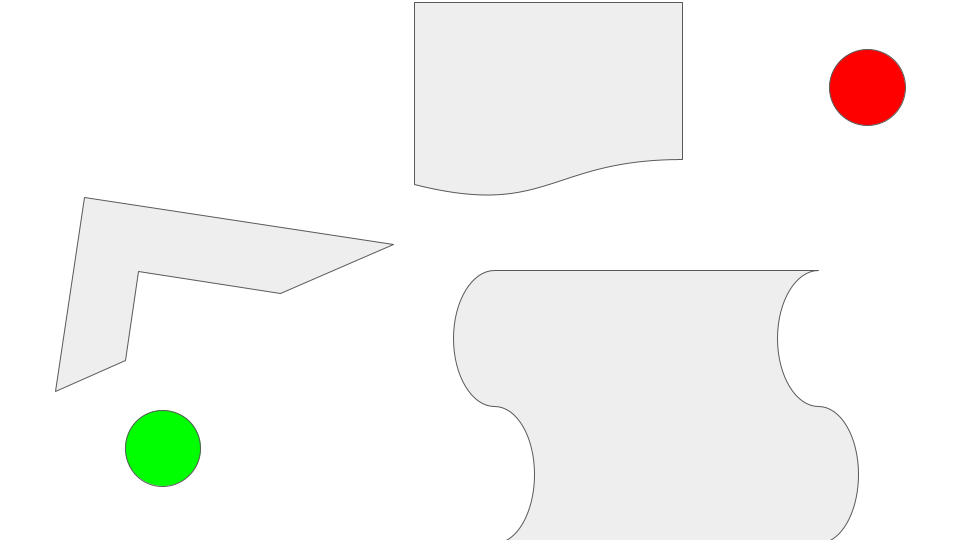
\includegraphics[width=\textwidth]{./assets/rrt_slides/rrt_slides_2.png}
\end{frame}

\begin{frame}{Example \textsc{sbmp} Execution: Sampling}
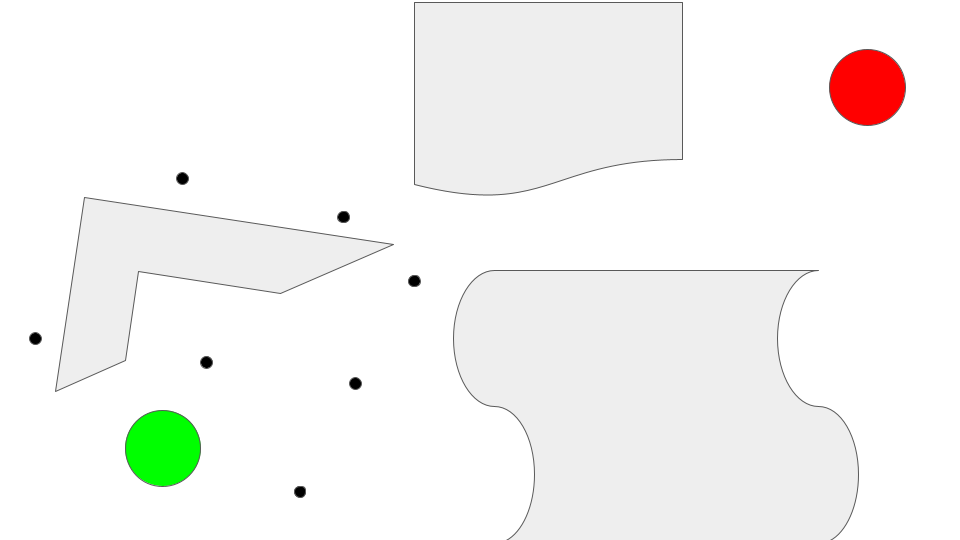
\includegraphics[width=\textwidth]{./assets/rrt_slides/rrt_slides_3.png}
\end{frame}

\begin{frame}{Example \textsc{sbmp} Execution: Local Planning}
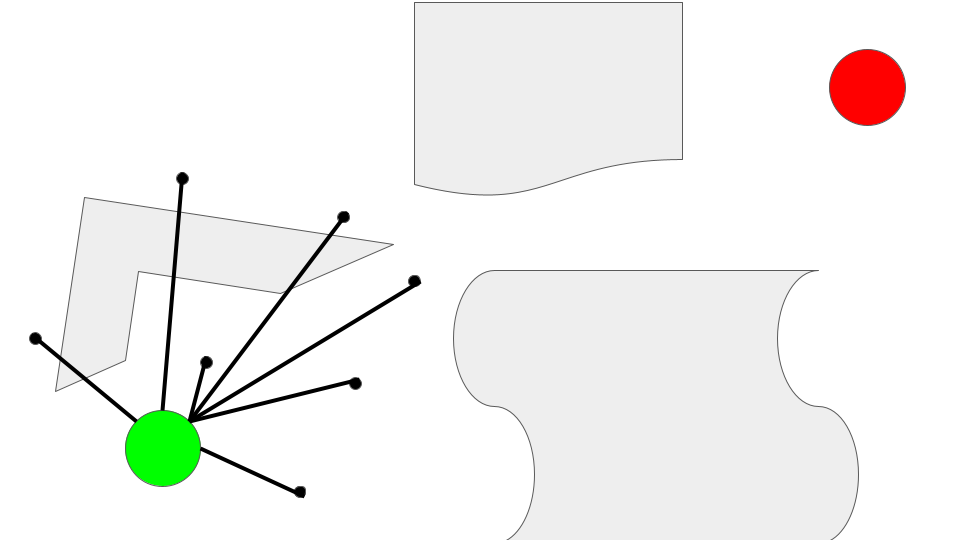
\includegraphics[width=\textwidth]{./assets/rrt_slides/rrt_slides_4.png}
\end{frame}

\begin{frame}{Example \textsc{sbmp} Execution: Collision Checking}
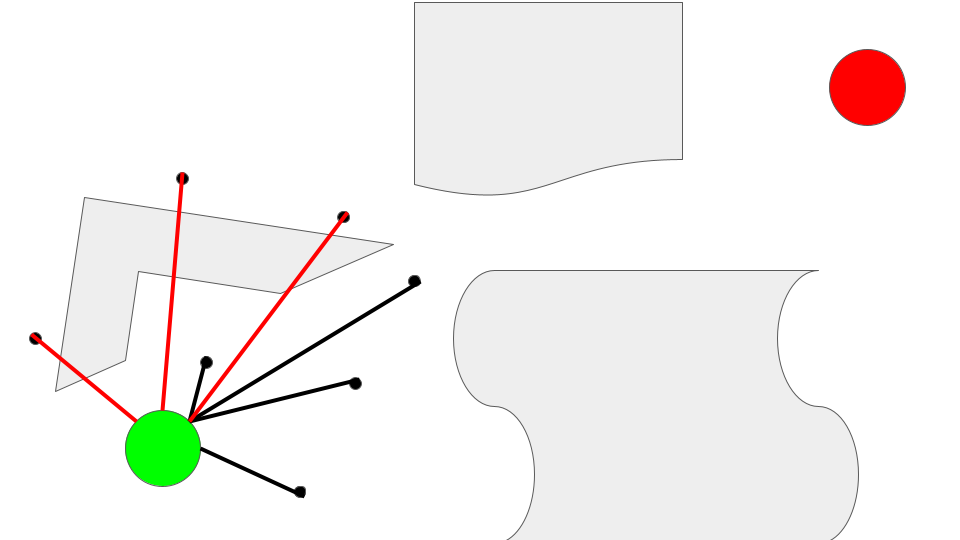
\includegraphics[width=\textwidth]{./assets/rrt_slides/rrt_slides_5.png}
\end{frame}

\begin{frame}{Example \textsc{sbmp} Execution: Motion Validation}
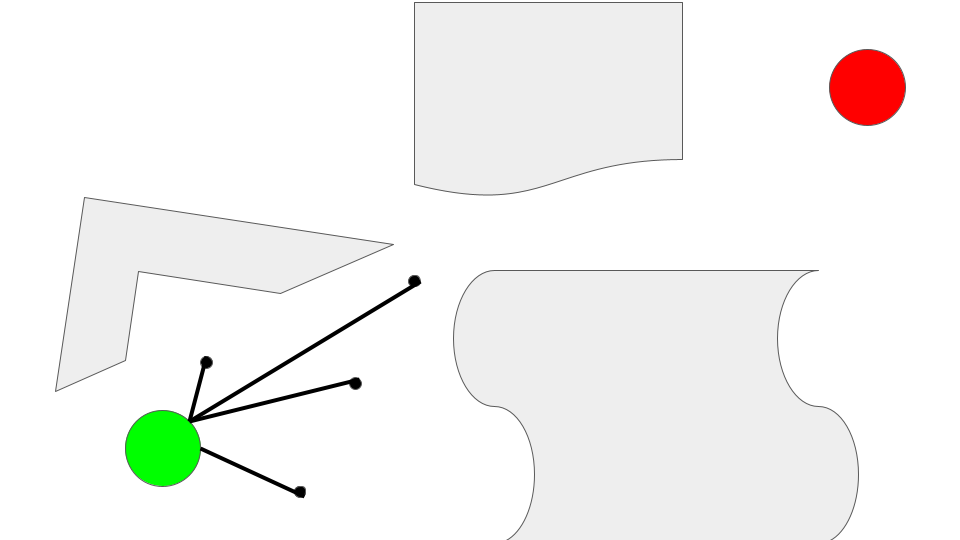
\includegraphics[width=\textwidth]{./assets/rrt_slides/rrt_slides_6.png}
\end{frame}

\begin{frame}{Example \textsc{sbmp} Execution: Generate Whole Graph}
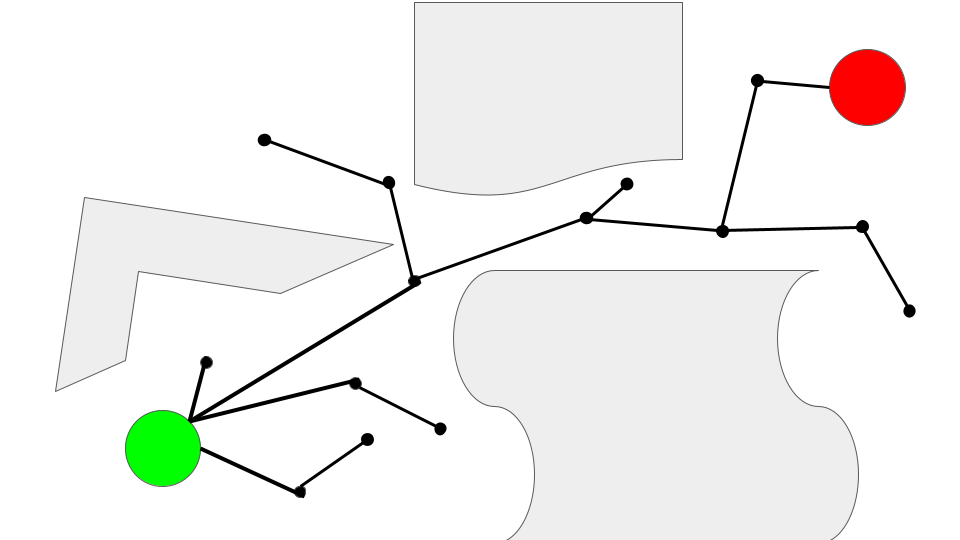
\includegraphics[width=\textwidth]{./assets/rrt_slides/rrt_slides_7.png}
\end{frame}

\begin{frame}{Example \textsc{sbmp} Execution: Find Path}
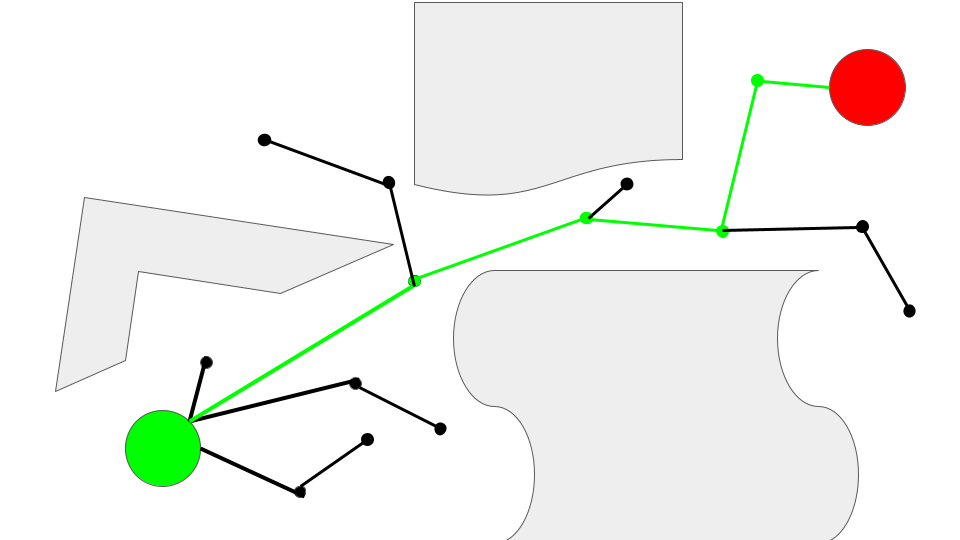
\includegraphics[width=\textwidth]{./assets/rrt_slides/rrt_slides_8.png}
\end{frame}

\end{document}